

\tikzset{every picture/.style={line width=0.75pt}} %set default line width to 0.75pt        

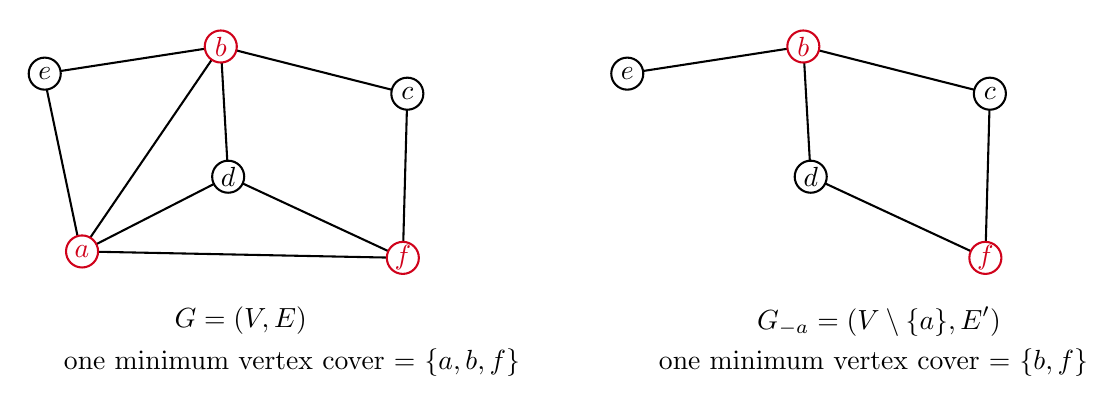
\begin{tikzpicture}[x=0.5pt,y=0.5pt,yscale=-1,xscale=1]
%uncomment if require: \path (0,258); %set diagram left start at 0, and has height of 258

%Straight Lines [id:da7485926733039977] 
\draw    (144.6,14.97) -- (43.43,163.09) ;
%Straight Lines [id:da4575120980127291] 
\draw [color={rgb, 255:red, 0; green, 0; blue, 0 }  ,draw opacity=1 ][line width=0.75]    (16.46,34.58) -- (143.69,14.97) ;
%Straight Lines [id:da9165715401778428] 
\draw    (16.46,34.58) -- (43.43,163.09) ;
%Straight Lines [id:da994182434786223] 
\draw [color={rgb, 255:red, 0; green, 0; blue, 0 }  ,draw opacity=1 ][line width=0.75]    (44.34,163.09) -- (276.17,167.73) ;
%Straight Lines [id:da9750224919648968] 
\draw    (149.95,109.07) -- (276.17,167.73) ;
%Straight Lines [id:da24348552449211425] 
\draw    (144.6,14.97) -- (149.95,109.07) ;
%Straight Lines [id:da16705340438790406] 
\draw    (144.6,14.97) -- (279.42,49.07) ;
%Straight Lines [id:da08663700279220432] 
\draw    (279.42,49.07) -- (276.17,167.73) ;
%Straight Lines [id:da4151454155794566] 
\draw    (149.95,109.07) -- (44.34,163.09) ;
%Shape: Ellipse [id:dp9133580928774087] 
\draw  [fill={rgb, 255:red, 255; green, 255; blue, 255 }  ,fill opacity=1 ] (5.79,34.58) .. controls (5.79,28.18) and (10.97,23) .. (17.37,23) .. controls (23.76,23) and (28.95,28.18) .. (28.95,34.58) .. controls (28.95,40.97) and (23.76,46.16) .. (17.37,46.16) .. controls (10.97,46.16) and (5.79,40.97) .. (5.79,34.58) -- cycle ;
%Shape: Ellipse [id:dp4005957609675306] 
\draw  [color={rgb, 255:red, 208; green, 2; blue, 27 }  ,draw opacity=1 ][fill={rgb, 255:red, 255; green, 255; blue, 255 }  ,fill opacity=1 ] (133.02,14.97) .. controls (133.02,8.57) and (138.2,3.39) .. (144.6,3.39) .. controls (151,3.39) and (156.18,8.57) .. (156.18,14.97) .. controls (156.18,21.36) and (151,26.55) .. (144.6,26.55) .. controls (138.2,26.55) and (133.02,21.36) .. (133.02,14.97) -- cycle ;
%Shape: Ellipse [id:dp49214617921702164] 
\draw  [fill={rgb, 255:red, 255; green, 255; blue, 255 }  ,fill opacity=1 ] (267.84,49.07) .. controls (267.84,42.67) and (273.02,37.49) .. (279.42,37.49) .. controls (285.82,37.49) and (291,42.67) .. (291,49.07) .. controls (291,55.46) and (285.82,60.65) .. (279.42,60.65) .. controls (273.02,60.65) and (267.84,55.46) .. (267.84,49.07) -- cycle ;
%Shape: Ellipse [id:dp8440754424343925] 
\draw  [fill={rgb, 255:red, 255; green, 255; blue, 255 }  ,fill opacity=1 ] (138.37,109.07) .. controls (138.37,102.68) and (143.55,97.49) .. (149.95,97.49) .. controls (156.34,97.49) and (161.53,102.68) .. (161.53,109.07) .. controls (161.53,115.47) and (156.34,120.65) .. (149.95,120.65) .. controls (143.55,120.65) and (138.37,115.47) .. (138.37,109.07) -- cycle ;
%Shape: Ellipse [id:dp20660183368429152] 
\draw  [color={rgb, 255:red, 208; green, 2; blue, 27 }  ,draw opacity=1 ][fill={rgb, 255:red, 255; green, 255; blue, 255 }  ,fill opacity=1 ] (32.76,163.09) .. controls (32.76,156.7) and (37.94,151.51) .. (44.34,151.51) .. controls (50.73,151.51) and (55.92,156.7) .. (55.92,163.09) .. controls (55.92,169.49) and (50.73,174.67) .. (44.34,174.67) .. controls (37.94,174.67) and (32.76,169.49) .. (32.76,163.09) -- cycle ;
%Shape: Ellipse [id:dp4098192910838151] 
\draw  [color={rgb, 255:red, 208; green, 2; blue, 27 }  ,draw opacity=1 ][fill={rgb, 255:red, 255; green, 255; blue, 255 }  ,fill opacity=1 ] (264.59,167.73) .. controls (264.59,161.33) and (269.77,156.15) .. (276.17,156.15) .. controls (282.56,156.15) and (287.75,161.33) .. (287.75,167.73) .. controls (287.75,174.13) and (282.56,179.31) .. (276.17,179.31) .. controls (269.77,179.31) and (264.59,174.13) .. (264.59,167.73) -- cycle ;
%Straight Lines [id:da21246297301250638] 
\draw [color={rgb, 255:red, 0; green, 0; blue, 0 }  ,draw opacity=1 ][line width=0.75]    (437.46,34.58) -- (564.69,14.97) ;
%Straight Lines [id:da5785088156918158] 
\draw    (570.95,109.07) -- (697.17,167.73) ;
%Straight Lines [id:da5748239667299] 
\draw    (565.6,14.97) -- (570.95,109.07) ;
%Straight Lines [id:da6918111132338757] 
\draw    (565.6,14.97) -- (700.42,49.07) ;
%Straight Lines [id:da17309311683158612] 
\draw    (700.42,49.07) -- (697.17,167.73) ;
%Shape: Ellipse [id:dp420664278746398] 
\draw  [fill={rgb, 255:red, 255; green, 255; blue, 255 }  ,fill opacity=1 ] (426.79,34.58) .. controls (426.79,28.18) and (431.97,23) .. (438.37,23) .. controls (444.76,23) and (449.95,28.18) .. (449.95,34.58) .. controls (449.95,40.97) and (444.76,46.16) .. (438.37,46.16) .. controls (431.97,46.16) and (426.79,40.97) .. (426.79,34.58) -- cycle ;
%Shape: Ellipse [id:dp5066222807713637] 
\draw  [color={rgb, 255:red, 208; green, 2; blue, 27 }  ,draw opacity=1 ][fill={rgb, 255:red, 255; green, 255; blue, 255 }  ,fill opacity=1 ] (554.02,14.97) .. controls (554.02,8.57) and (559.2,3.39) .. (565.6,3.39) .. controls (572,3.39) and (577.18,8.57) .. (577.18,14.97) .. controls (577.18,21.36) and (572,26.55) .. (565.6,26.55) .. controls (559.2,26.55) and (554.02,21.36) .. (554.02,14.97) -- cycle ;
%Shape: Ellipse [id:dp33896202753015414] 
\draw  [fill={rgb, 255:red, 255; green, 255; blue, 255 }  ,fill opacity=1 ] (688.84,49.07) .. controls (688.84,42.67) and (694.02,37.49) .. (700.42,37.49) .. controls (706.82,37.49) and (712,42.67) .. (712,49.07) .. controls (712,55.46) and (706.82,60.65) .. (700.42,60.65) .. controls (694.02,60.65) and (688.84,55.46) .. (688.84,49.07) -- cycle ;
%Shape: Ellipse [id:dp43743104841029357] 
\draw  [fill={rgb, 255:red, 255; green, 255; blue, 255 }  ,fill opacity=1 ] (559.37,109.07) .. controls (559.37,102.68) and (564.55,97.49) .. (570.95,97.49) .. controls (577.34,97.49) and (582.53,102.68) .. (582.53,109.07) .. controls (582.53,115.47) and (577.34,120.65) .. (570.95,120.65) .. controls (564.55,120.65) and (559.37,115.47) .. (559.37,109.07) -- cycle ;
%Shape: Ellipse [id:dp7957741048650372] 
\draw  [color={rgb, 255:red, 208; green, 2; blue, 27 }  ,draw opacity=1 ][fill={rgb, 255:red, 255; green, 255; blue, 255 }  ,fill opacity=1 ] (685.59,167.73) .. controls (685.59,161.33) and (690.77,156.15) .. (697.17,156.15) .. controls (703.56,156.15) and (708.75,161.33) .. (708.75,167.73) .. controls (708.75,174.13) and (703.56,179.31) .. (697.17,179.31) .. controls (690.77,179.31) and (685.59,174.13) .. (685.59,167.73) -- cycle ;

% Text Node
\draw (17.37,34.58) node   [align=left] {$\displaystyle e$};
% Text Node
\draw (144.6,14.97) node  [color={rgb, 255:red, 208; green, 2; blue, 27 }  ,opacity=1 ] [align=left] {$\displaystyle b$};
% Text Node
\draw (279.42,49.07) node   [align=left] {$\displaystyle c$};
% Text Node
\draw (149.95,109.07) node   [align=left] {$\displaystyle d$};
% Text Node
\draw (44.34,163.09) node  [color={rgb, 255:red, 208; green, 2; blue, 27 }  ,opacity=1 ] [align=left] {$\displaystyle a$};
% Text Node
\draw (276.17,167.73) node  [color={rgb, 255:red, 208; green, 2; blue, 27 }  ,opacity=1 ] [align=left] {$\displaystyle f$};
% Text Node
\draw (109,201) node [anchor=north west][inner sep=0.75pt]   [align=left] {$\displaystyle G=( V,E)$};
% Text Node
\draw (438.37,34.58) node   [align=left] {$\displaystyle e$};
% Text Node
\draw (565.6,14.97) node  [color={rgb, 255:red, 208; green, 2; blue, 27 }  ,opacity=1 ] [align=left] {$\displaystyle b$};
% Text Node
\draw (700.42,49.07) node   [align=left] {$\displaystyle c$};
% Text Node
\draw (570.95,109.07) node   [align=left] {$\displaystyle d$};
% Text Node
\draw (697.17,167.73) node  [color={rgb, 255:red, 208; green, 2; blue, 27 }  ,opacity=1 ] [align=left] {$\displaystyle f$};
% Text Node
\draw (530,201) node [anchor=north west][inner sep=0.75pt]   [align=left] {$\displaystyle G_{-a} =( V\setminus \{a\} ,E')$};
% Text Node
\draw (29,231) node [anchor=north west][inner sep=0.75pt]   [align=left] {one minimum vertex cover = $\displaystyle \{a,b,f\}$};
% Text Node
\draw (459,231) node [anchor=north west][inner sep=0.75pt]   [align=left] {one minimum vertex cover = $\displaystyle \{b,f\}$};


\end{tikzpicture}

